% !TEX program = pdflatex
% !TEX enableSynctex = true
\documentclass[aspectratio=169,10pt]{beamer}

%%%%%%%%%%%%%%%
\usepackage{booktabs}
\usepackage{xspace}
\usepackage{ulem}
\usepackage{subfig}
\usepackage{graphicx}
\usepackage{xcolor}
\usepackage{multirow}
\usepackage[capitalise,noabbrev]{cleveref} 
\usepackage{datatool}
\usepackage{algorithm} 
\usepackage{algpseudocode} 
\usepackage{empheq}
\usepackage[many]{tcolorbox}
\usepackage[capitalise,noabbrev]{cleveref}
\usetheme[progressbar=frametitle,block=fill]{metropolis}

\newcommand{\themename}{\textbf{\textsc{metropolis}}\xspace}
\definecolor{emphcolorval}{rgb}{0.23,0.4,0.7}
\definecolor{highlightcolorval}{rgb}{1,0,0}
% Penn colors
\definecolor{PennRed}{RGB}{149, 0, 26}
\definecolor{PennBlue}{RGB}{1, 37, 110}

\setbeamercolor{frametitle}{bg=PennBlue}
\setbeamercolor{progress bar}{fg=PennBlue}
\setbeamercolor{math text}{fg=PennRed}

\setbeamercolor{block title}{fg=PennBlue}
\setbeamercolor{block body}{fg=PennBlue}

\setbeamercolor{block title example}{fg=PennBlue}
\setbeamercolor{block body example}{fg=PennBlue, bg=yellow}

\setbeamersize{text margin left=5.5pt, text margin right=5.5pt}

\definecolor{cosmiclatte}{rgb}{1.0, 0.99, 0.95}
\setbeamercolor{background canvas}{bg=cosmiclatte}
%\titlegraphic{\hfill\includegraphics[height=0.8cm]{/Users/jesusfv/dropbox/Templates_Slides/penn_fulllogo.pdf}}
\newcommand{\emphcolor}[1]{\textbf{\textcolor{emphcolorval}{#1}}}
%\newcommand{\mathcolor}[1]{{\mathbf{\color{emphcolorval}{#1}}}}
\newcommand{\highlightcolor}[1]{{\textbf{\color{highlightcolorval}{#1}}}}

% \usepackage{natbib}
% \bibliographystyle{ecta}

\crefname{equation}{}{}
\newtheorem{proposition}{Proposition}
\newcommand\bigzero{\makebox(0,0){\text{\huge0}}}
\newcommand{\D}[1][]{\ensuremath{\boldsymbol{\partial}_{#1}}}
\newcommand{\R}{\ensuremath{\mathbb{R}}}
\newcommand{\diff}{\ensuremath{\mathrm{d}}}
\newcommand{\ex}{\ensuremath{\mathrm{ex}}}
\newcommand{\set}[1]{\ensuremath{\left\{{#1}\right\}}}
\newcommand{\indicator}[1]{\ensuremath{\mathds{1}\left\{{#1}\right\}}}
\newcommand{\condexpec}[3][]{\ensuremath{\mathbb{E}_{#1}\left[{#2} \; \middle| \; {#3} \right]}}
\newcommand{\prob}[2][]{\ensuremath{\mathbb{P}_{#1}\left( {#2} \right)}}
\newcommand{\cprob}[2]{\ensuremath{\mathbb{P}\left( {#1}\left| {#2} \right. \right)}}
\newcommand{\condcov}[2]{\ensuremath{\mathrm{cov}\left({#1} \; \middle| \; {#2} \right)}}
\newcommand{\expec}[2][]{\ensuremath{\mathbb{E}_{{#1}}\left[ {#2} \right]}}
\newcommand{\bigO}[1]{\ensuremath{\mathcal{O}(#1)}}
\newcommand{\Xdom}{\mathcal{X}}
\newcommand{\Yrange}{\mathcal{Y}}
\newcommand{\Xtrain}{\mathcal{X}_{\mathrm{train}}}
\newcommand{\Xextr}{\mathcal{X}_{\mathrm{extr}}}
\newcommand{\Xhull}{\mathrm{Hull}(\Xtrain)}
\newcommand{\Xtest}{\mathcal{X}_{\mathrm{test}}}
\newcommand{\Ltest}{\ell_{\mathrm{test}}}
\newcommand{\F}{\mathcal{F}}
\newcommand{\Resid}{\mathcal{R}}
\newcommand{\st}{\textrm{s.t.}\,}

\begin{document}
\title{{\vspace{0.4in}\hspace{0.2in}\textcolor{PennBlue}{Spooky Boundaries at a Distance: \\ \hspace*{5 mm}Inductive Bias, Dynamic Models, and Behavioral Macro}}}
\author{\hspace*{4 mm} Mahdi Ebrahimi Kahou\inst{1}\and
	Jes\'{u}s Fern\'{a}ndez-Villaverde\inst{2} \and Sebasti\'an G\'omez-Cardona\inst{3} \\ \hspace*{4 mm}  Jesse Perla\inst{4} \and Jan Rosa\inst{4}}

\institute{ \inst{\bf \hspace{0.2in} Conference on Frontiers in Machine Learning and Economics, Federal Reserve Bank of Philadelphia } \and
	\inst{\hspace{0.2in}1}Bowdoin College\and
	\inst{\hspace{0.2in}2}University of Pennsylvania \and
	\inst{\hspace{0.2in}3}Morningstar, Inc. \and
	\inst{\hspace{0.2in}4} University of British Columbia}


\date{}

\maketitle

\section{\textcolor{PennBlue}{Motivation, Question, and Contribution}}

\begin{frame}{Motivation}
	\begin{center}
		\emphcolor{In the long run, we are all dead---{\it J.M. Keynes, A Tract on Monetary Reform (1923)}}
		%I  will come back to this couple of time during the talk
	\end{center}
	\begin{itemize}
		\item Numerical solutions to dynamical systems are central to many quantitative fields in economics.
		% such as macroeconomics, empirical Industrial organization, urban economics, and spatial economics
		\vspace{0.1in}
		\item Many dynamical systems in economics are \emphcolor{boundary value} problems:
		%unlike mnay problems natural sciences and engineering :
		\vspace{0.1in}
		\begin{enumerate}
				\item The boundary is at \emphcolor{infinity}.
				\vspace{0.05in}
				\item The values at the boundary are potentially \emphcolor{unknown}.
				\vspace{0.05in}  
		\end{enumerate}
		\item Resulting from \emphcolor{forward looking} behavior of agents.
		% and it is requirement for optimality
		\vspace{0.1in}
		\item Examples include the \emph{{\it transversality}} and the \emph{\it  no-bubble} condition.
		% No ponzi scheme
		\vspace{0.1in}
		\item Without them, the problems are \emphcolor{ill-posed} and have infinitely many solutions: 
		\vspace{0.1in}
		\begin{itemize}
			\item The problems are ill-posed in the Hadamard sense, meaning the solutions are not unique.
			\item These forward-looking boundary conditions are a key limitation on increasing dimensionality.
		\end{itemize}
			% what do I mean by that, if it wasnt a boundary condition at infinity, I could easily solve a 1000 dimensional initial value problem 
	\end{itemize}
\end{frame}


\begin{frame}{Question}
	\emphcolor{Question}:
	\hspace{200mm}
	
	\begin{quote}
			Can we (economists and agents) \emphcolor{ignore} these long-run boundary conditions and still have accurate short/medium-run dynamics disciplined by these long-run conditions?
	\end{quote}
\end{frame}



\begin{frame}{Contribution}
	
\begin{enumerate}
	\item \emphcolor{Yes}, it is possible to meet
	long-run boundary conditions \emphcolor{without} strictly enforcing them as a constraint on the model’s dynamics.
	\vspace{0.05in}
	\begin{itemize}
		\item We show how using Machine Learning (ML) methods achieve this.
		\vspace{0.025in}
		\item This is due to the \emphcolor{inductive bias} of ML methods.
		\vspace{0.025in} 
		\item In this paper focusing on \emph{deep neural networks}
		\vspace{0.025in} 
	\end{itemize} 
	\item We argue the inductive bias provides a foundation for modeling forward-looking behavioral
	agents with self-consistent expectations.
	\vspace{0.025in}
	\begin{itemize}
		\item Easy to compute. 
		\vspace{0.025in}
		\item Provides short-run accuracy.
		\vspace{0.025in}
		\item Satisfies the necessary long-run constraints.
	\end{itemize}
\end{enumerate}

\end{frame}

\section{\textcolor{PennBlue}{Background: Economic Models, Deep learning and inductive bias}}


\begin{frame}
	\frametitle{Economic Models: functional equations}
	Many theoretical models can be written as functional equations:
	\begin{itemize}
		\item Economic object of interest: $f $, where $f : \Xdom\to \mathcal{R}\subseteq \mathbb{R}^N$ 
		\begin{itemize}
			\item e.g., asset price, investment choice, best-response, etc.
		\end{itemize}
			\vspace{0.1in}
		\item Domain of $f$: $\Xdom$  
		\begin{itemize}
			\item e.g. space of dividends, capital, opponents state or time in sequential models.
		\end{itemize}
			\vspace{0.1in}
		\item The ``model'' error:  $\ell \big(x,f\big) = \mathbf{0}$,  for all $x\in \Xdom$  
		\begin{itemize}
			\item e.g., Euler and Bellman residuals, equilibrium FOCs.
		\end{itemize}
		\vspace{0.1in}
	\end{itemize}
	Then a \emphcolor{solution} is an $f^*\in \F$ where $\ell(x,f^*) = \mathbf{0}$ for all $x \in \Xdom$.\vspace{0.1in}
\end{frame}

\begin{frame}{Approximate solution: deep neural networks }
	\begin{enumerate}
		\item Sample $\mathcal{X}$: $\mathcal{D} = \{x_1,\cdots,x_N\}$
		\vspace{0.025in}
		\item Pick a deep neural network $f_\theta(\cdot) \in \mathcal{H}(\theta)$:
		\begin{itemize}
			\item $\theta$: parameters for optimization (i.e., weights and biases).  
		\end{itemize}
		\vspace{0.025in}
		\item To find an approximation for $f$ solve:
		\begin{align*}
			\min_{\theta } \frac{1}{N}\sum_{x \in \mathcal{D}} \|\underbrace{\ell(x,f_\theta)}_{\text{Econ model error}}\|_2^2
		\end{align*}
		\begin{itemize}
			\item Deep neural networks are highly over-parameterized.
			\item Formally, $|\theta|\gg N$ 
		\end{itemize}
	\end{enumerate}
\end{frame}

\begin{frame}{Over-parameterized interpolation}
	\begin{itemize}
		\item Over-parameterized ($|\theta|\gg N$), the optimization problem can have many solutions.
		\item Since individual $\theta$ are irrelevant it is helpful to think of optimization directly within $\mathcal{H}$
		\vspace{-0.025in}
		\begin{empheq}[box=\tcbhighmath]{equation*}
			\min_{f_{\theta} \in \mathcal{H}} \frac{1}{N}\sum_{x \in \mathcal{D}} \|\ell(x,f_{\theta})\|_2^2\label{eq:functional-optimization}
		\end{empheq}
		\vspace{-0.025in}
	\item But which $f_{\theta}$?
	\item \emphcolor{Mental model:} chooses min-norm interpolating solution for a (usually) unknown functional norm $\psi$
			\vspace{-0.025in}
	\begin{empheq}[box=\tcbhighmath]{align*}
		\min_{f_\theta\in \mathcal{H}} &||f_\theta||_\psi\\
		\st & \ell(x,f_\theta)=0,\quad \text{ for all } x \in \mathcal{D}
	\end{empheq}
	\vspace{-0.025in}
	\item That is what we mean by \emphcolor{inductive bias} (see Belkin, 2021 and Ma and Yang, 2021).
	
	\item  Characterizing $S$ (e.g., Sobolev norms or semi-norms?) is an active research area in ML.
	\end{itemize}
\end{frame}

\begin{frame}{Smooth interpolation}
	\begin{itemize}
		\item Intuition: biased toward solutions which are flattest and have smallest derivatives
	\end{itemize}
		\begin{figure}[t!]
		\centering
		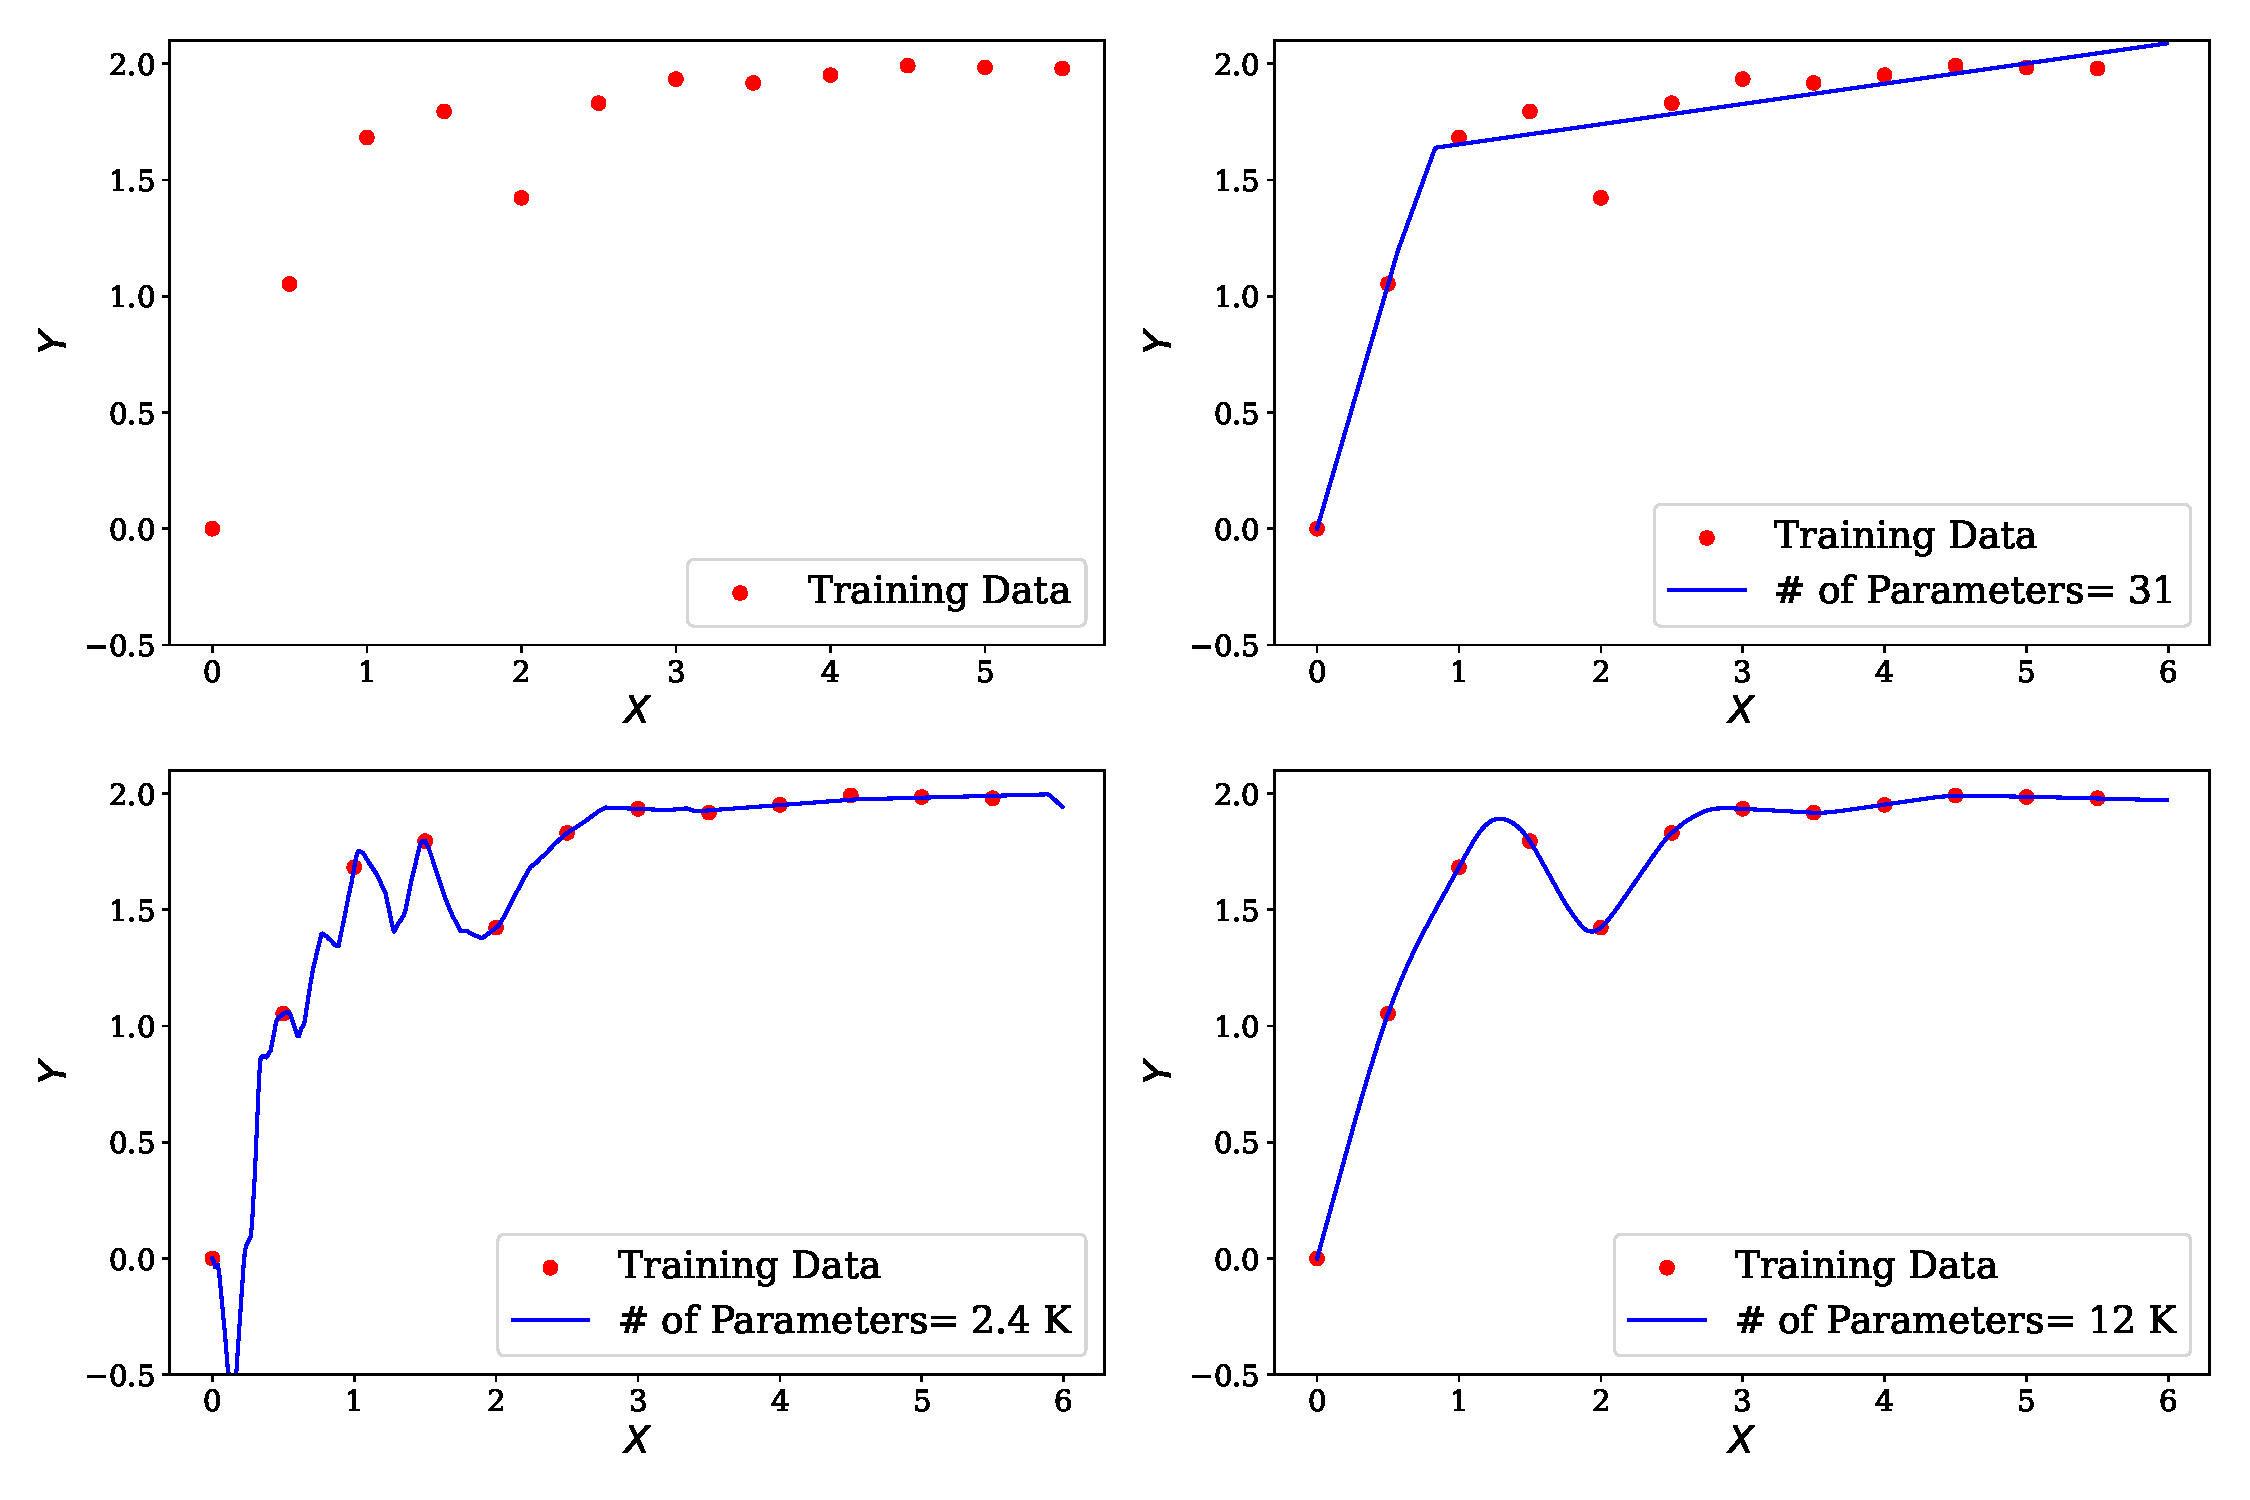
\includegraphics[width=0.65\textwidth]{figs/smooth_interpolation.pdf}
	\end{figure}
\end{frame}

\begin{frame}{Intuition of the paper}
	\begin{columns}
		\begin{column}{0.5\textwidth}
			% Content for the left column
			\begin{itemize}
				\item \emphcolor{Minimum-norm inductive bias}: 
				\begin{itemize}
					\item Over-parameterized models (e.g., large neural networks) interpolate the train data.
					%therefore they are many possible solutions
					\vspace{0.05in}
					\item They are biased towards interpolating functions with smaller norms. 
					\item So they dont like explosive functions.
				\end{itemize}
				\vspace{0.1in}
				\item \emphcolor{Violation of economic boundary conditions}:
				\begin{itemize}
					\item Sub-optimal solutions diverge (explode) over time.
					% As you can see in the plot optimal solution goe to the steady-state, the black dot, and any othe trajectory globaly or locally diveges. That is the signature of economic models
					\vspace{0.05in}
					%\item They have large or explosive norms.
					% Given that they are divergent, then they are large functions with large norms
					\vspace{0.05in}
					\item This is due to the \emphcolor{saddle-path} nature of econ problems.
					% many economic models have this saddle path nature
					\vspace{0.05in}
					\item ``{\it Knife-edge stability is a common property of dynamic monetary models ...}" \textcolor{red}{Obstfeld and Rogoff (1983)} 
				\end{itemize}
			\end{itemize}
		\end{column}
		\begin{column}{0.5\textwidth}
		\begin{figure}[t!]
			\centering
			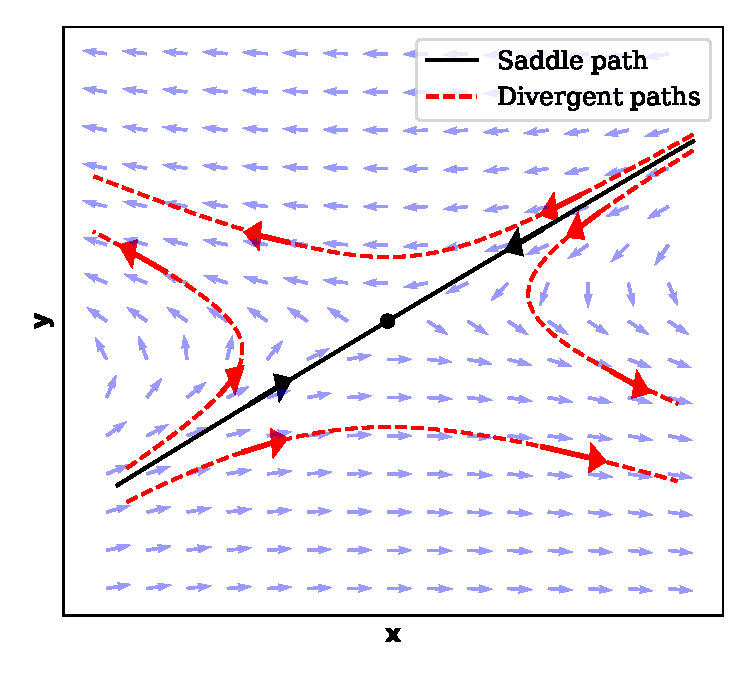
\includegraphics[width=\textwidth]{figs/saddle_path.pdf}
			\vspace{-7mm}
		\end{figure}
		\end{column}
	\end{columns}
\end{frame}

\section{Outline}

\begin{frame}{Outline of the Talk}
	
	To explore how we can ignore events after ``we are all dead'', we show deep learning solutions to
	\begin{enumerate}
		\item Classic linear-asset pricing model.\vspace{0.1in}
		\item Sequential formulation of the neoclassical growth model.\vspace{0.1in}
		\item Sequential formulation of the neoclassical growth model with non-concave production function.\vspace{0.1in}
		\item Equivalent for a recursive formulation of the neoclassical growth model.\vspace{0.1in}
		
	\end{enumerate}
\end{frame}

\section{\textcolor{PennBlue}{Linear asset pricing and the no-bubble condition}}

\begin{frame}{Linear asset pricing: setup }
	\begin{itemize}
	\item The risk-neutral price, $p(t)$, of a claim to a stream of dividends, $y(t)$, is given by
	the recursive equation:
	\begin{align*}
		p(t) = y(t) + \beta p(t+1), \quad \text{for}~ t=0,1,\cdots
	\end{align*}
	\item $\beta<1$, and $y(t)$ is exogenous, $y(0)$ given.
	\item  This is a two dimensional dynamical system with unknown initial condition  $p(0)$. This problem is \emphcolor{ill-posed}.
	\item A family of solutions
	 \begin{empheq}[box=\tcbhighmath]{align*}
	 	p(t) = \underbrace{p_f(t)}_{\text{fundamentals}} +  \underbrace{\zeta \left(\frac{1}{\beta}\right)^t}_{\text{explosive bubble}}
	 \end{empheq}
	 \item $p_f(t) \equiv \sum_{\tau =0}^\infty \beta^\tau y(t+\tau)$. Each solution corresponds to a different $\zeta>0$.
	\end{itemize}
\end{frame}


\begin{frame}{Linear asset pricing: the long-run boundary condition}
	\begin{columns}
		\begin{column}{0.5\textwidth}
			% Content for the left column
			\begin{itemize}
				\item Long-run boundary condition that rule out the explosive bubbles and chooses $\zeta =0$
				\begin{align*}
					\lim_{t\rightarrow \infty} \beta^t p(t) = 0.
				\end{align*}
				\vspace{0.1in}
				\item Any norm that preserve monotonicity, like $L_p$ and Sobolev (semi-)norms 
				\begin{align*}
					\min_{\zeta\geq 0} \|p\|_\psi = \|p_f\|_\psi
				\end{align*}
				\item Ignoring the no-bubble condition and using a deep neural network provides an accurate approximation for $p_f(t)$.
			\end{itemize}
		\end{column}
		\begin{column}{0.5\textwidth}
			\begin{figure}[t!]
				\centering
				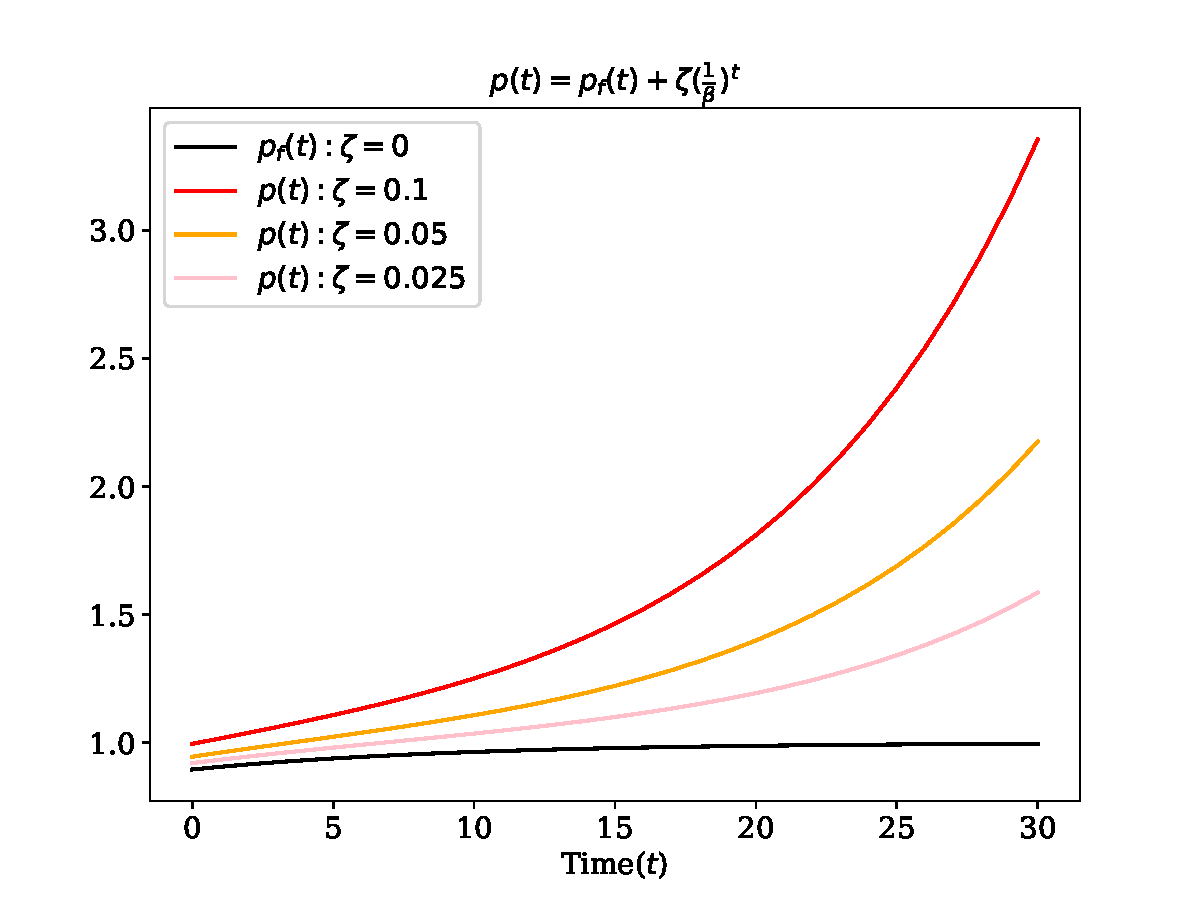
\includegraphics[width=\textwidth]{figs/bubble_solution.pdf}
				\vspace{-7mm}
			\end{figure}
		\end{column}
	\end{columns}
\end{frame}



\begin{frame}{Linear asset pricing: numerical method}
	\begin{itemize}
		\item Sample for time:  $\mathcal{D} = \{t_1,\cdots,t_N\}$.
		\item Dividend process: $y(t+1) = c+(1+g)y(t)$, given $y(0)$.
		\item A over-parameterized neural network $p_\theta(t)$, \emphcolor{ignore} the non-bubble condition and solve 
				\begin{empheq}[box=\tcbhighmath]{align*}
				\min_{\theta} \frac{1}{N}\sum_{t \in \mathcal{D}} \left[p_\theta(t)- y(t)- \beta p_\theta(t+1)\right]^2
			\end{empheq}
		\item This minimization should provide an accurate short- and medium-run approximation for price based on the fundamentals $p_f(t)$.
	\end{itemize}
	
\end{frame}
\begin{frame}{Linear asset pricing: results}
	\begin{columns}
		\begin{column}{0.5\textwidth}
			% Content for the left column
			\begin{itemize}
				\item Two cases: $g<0$ and $g>0$.
				\vspace{0.05in}
				\item Relative errors: $\varepsilon_p(t)\equiv \frac{p_\theta(t)-p_f(t)}{p_f(t)}$.
				\vspace{0.05in}
				\item for $g>0$: $p_\theta(t) = e^{\phi t}
			 NN_\theta(t)$, $\phi$ is "learnable".
			 	\vspace{0.05in}
				\item Results for $100$ different seeds (initialization of the parameters):
				\begin{itemize}
					\item important for non-convex optimizations.
				\end{itemize} 
				\vspace{0.05in}
				\item Very accurate short- and medium-run approximation.
			\end{itemize}
		\end{column}
		\begin{column}{0.5\textwidth}
			\begin{figure}[t!]
				\centering
				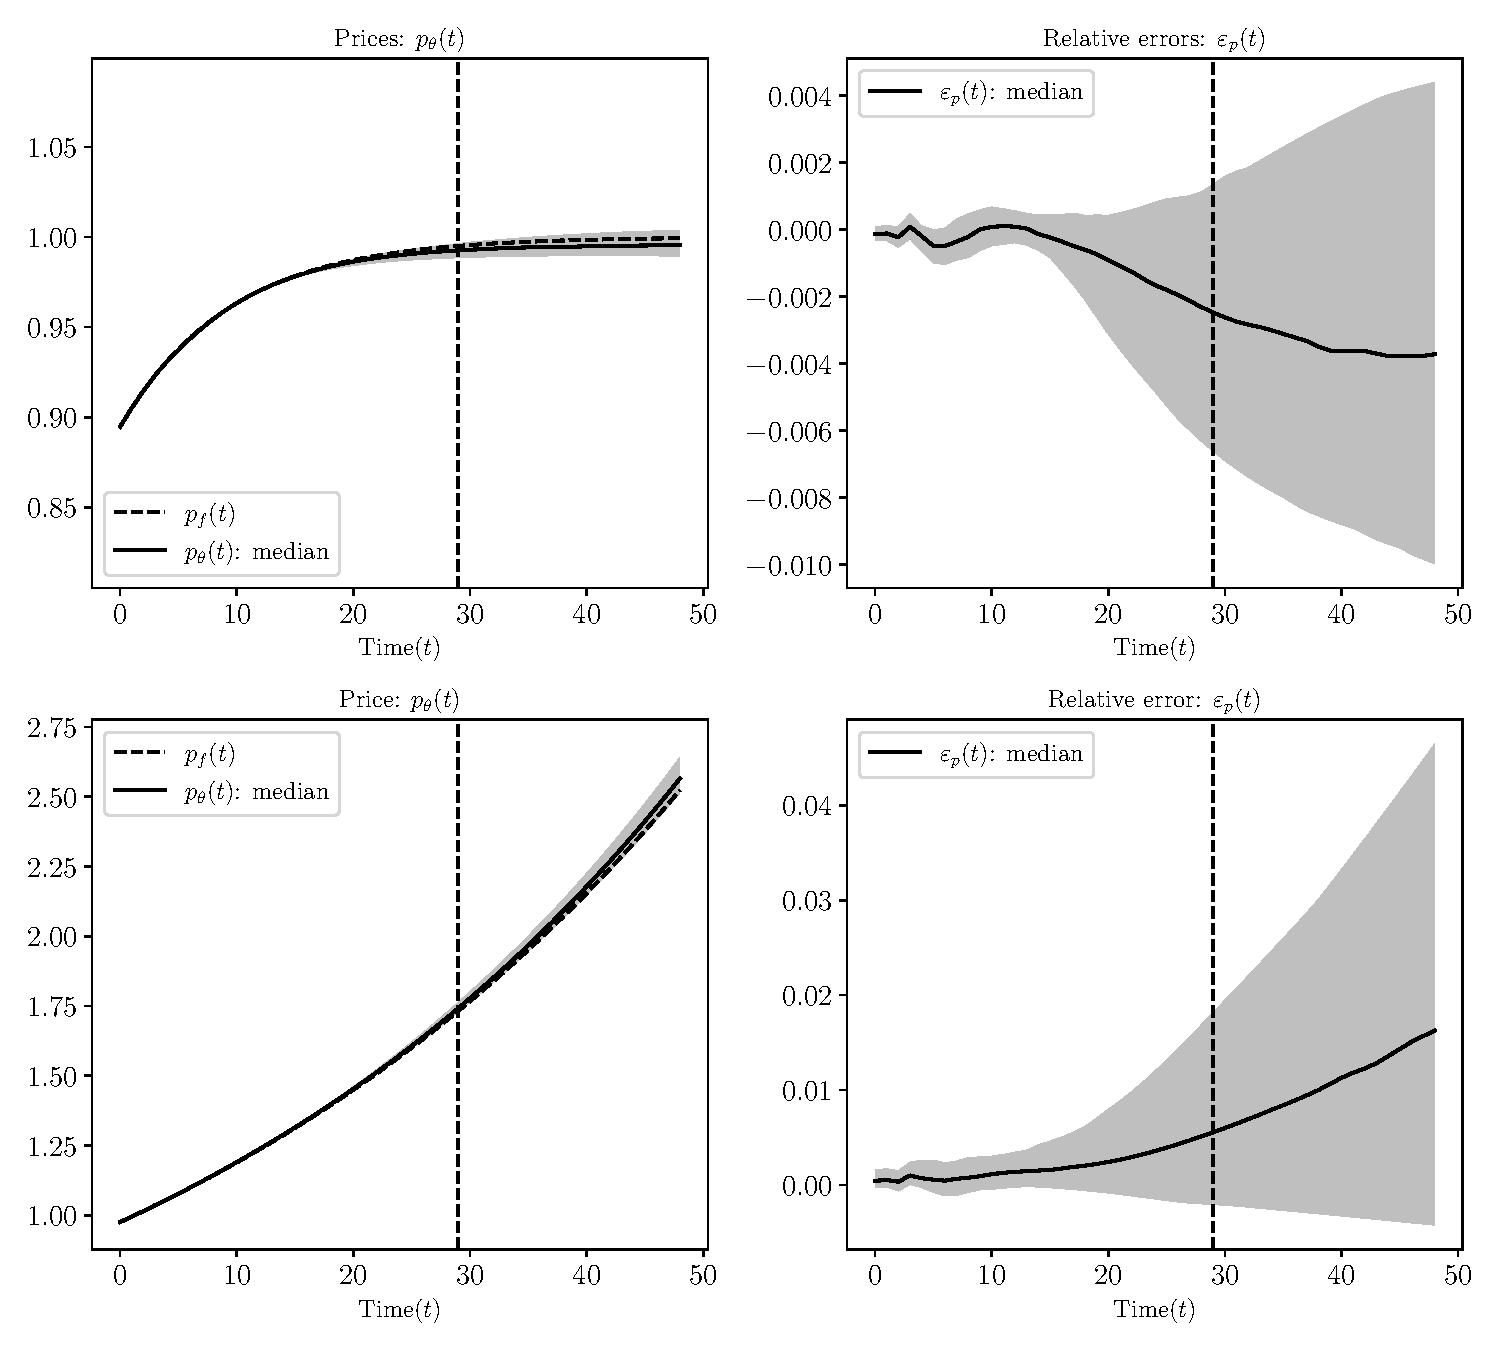
\includegraphics[width=\textwidth]{figs/asset_pricing_sequential_combined.pdf}
				\vspace{-7mm}
			\end{figure}
		\end{column}
	\end{columns}
\end{frame}




\begin{frame}{Neoclassical growth model: setup }
	\begin{itemize}
		\item Total factor productivity $z(t)$ exogenously given, capital $k(t)$ with given $k(0)$, consumption $c(t)$, production function $f(\cdot)$, depreciation rate $\delta<1$, discount factor $\beta$  :
		\begin{align*}
			&\underbrace{k(t+1) = z(t)^{1-\alpha} f\left(k(t)\right)+ (1-\delta)k(t)-c(t)}_{\text{feasibility constraint}}, \\ 
			&\underbrace{c(t+1) = \beta c(t) \left[z(t+1)^{1-\alpha}f'\big(k(t+1)\big)+1-\delta\right]}_{\text{Euler equation}}.
		\end{align*}
	\item This is a three dimensional dynamical system with unknown initial condition  $c(0)$. This problem is \emphcolor{ill-posed}.
	\vspace{0.05in}
	\item A family of solutions, each solution corresponds to a different $c(0)$.
	\end{itemize}	
\end{frame}

\begin{frame}{Neoclassical growth model: the long-run boundary condition}
	\begin{columns}
		\begin{column}{0.5\textwidth}
			% Content for the left column
			\begin{itemize}
				\item To rule out sub-optimal solutions, transversality condition
				\begin{align*}
					\lim_{t\rightarrow \infty}\beta^t \frac{k(t+1)}{c(t)} = 0
				\end{align*}
				\vspace{0.1in}
				\item  using a deep neural network and ignoring the transversality condition provides a an accurate approximation for the optimal capital path.
			\end{itemize}
		\end{column}
		\begin{column}{0.5\textwidth}
			\begin{figure}[t!]
				\centering
				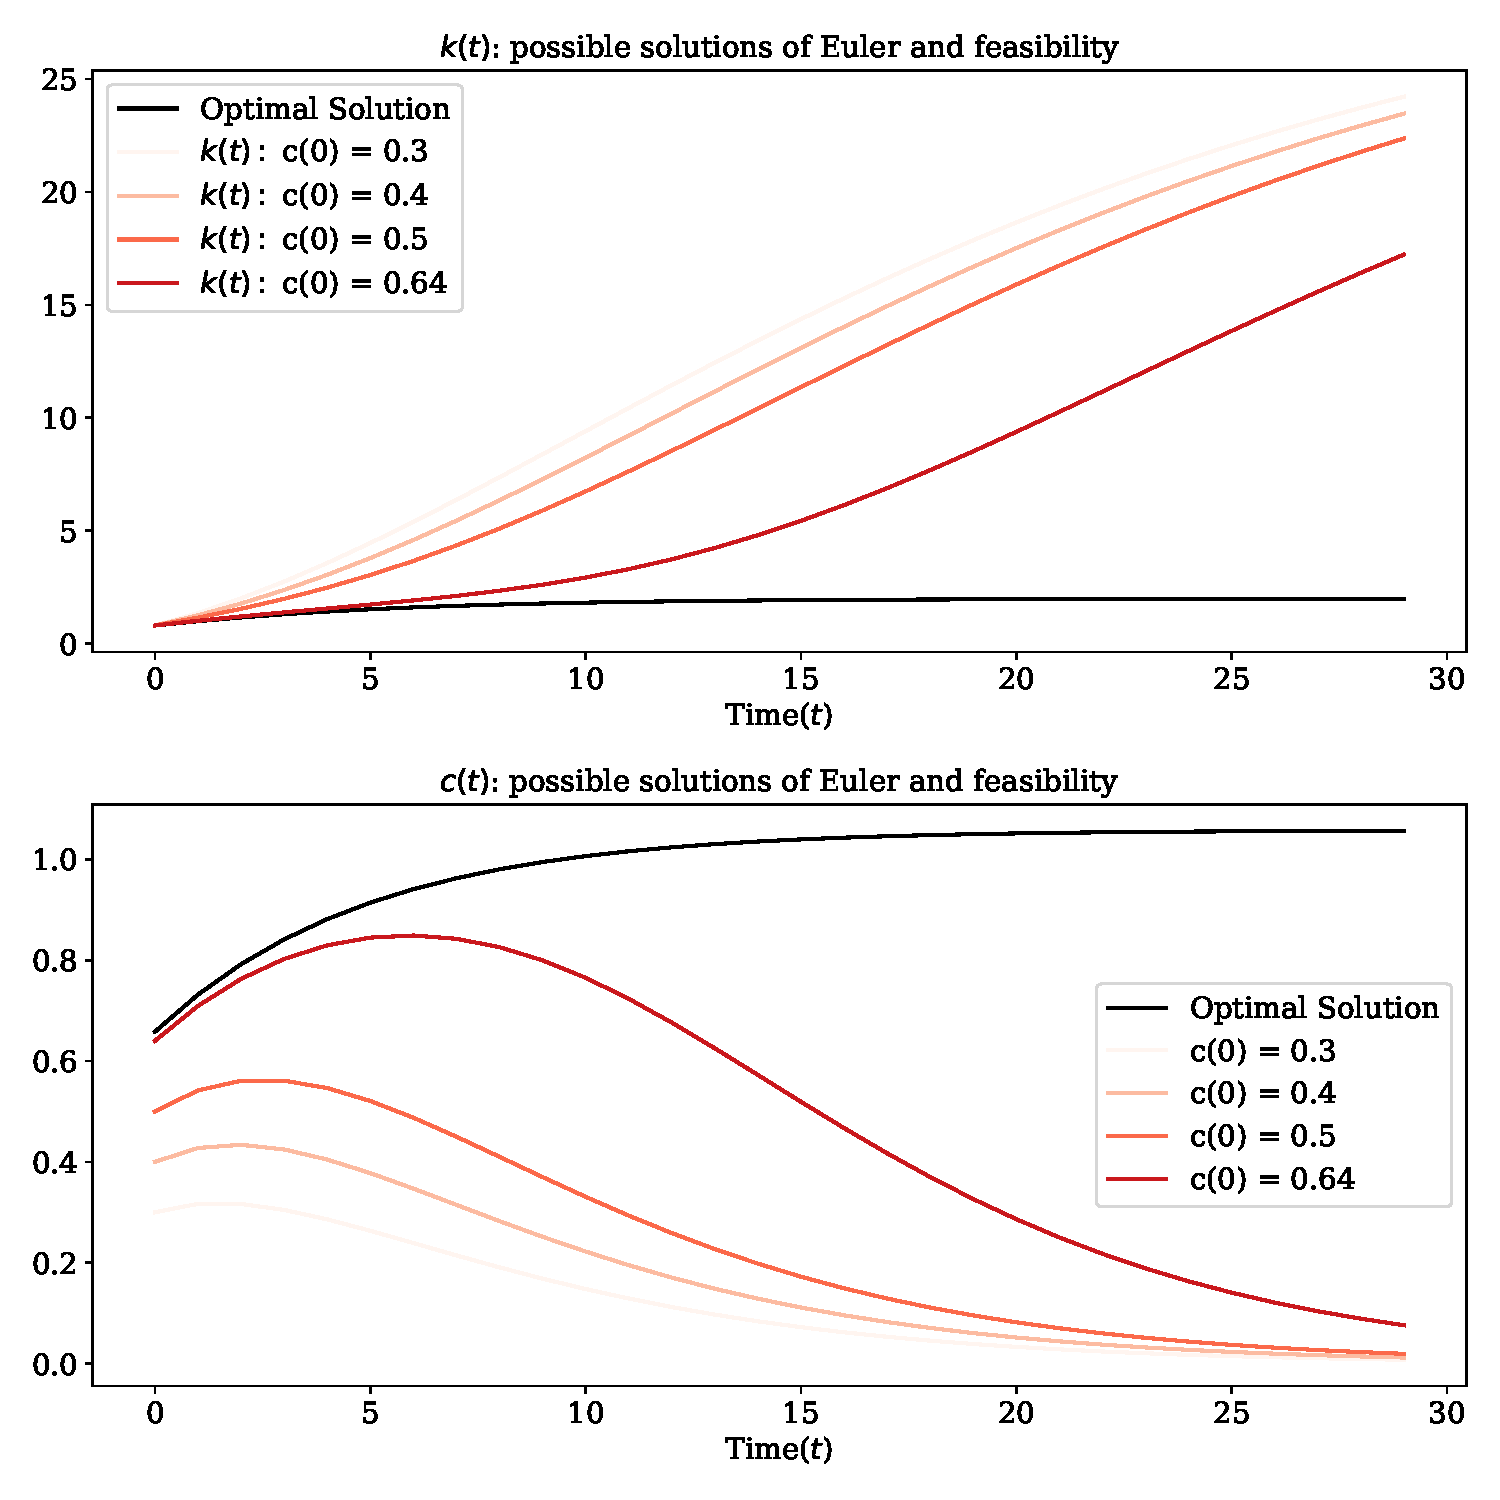
\includegraphics[width=0.6\textwidth]{figs/TVC_violation.pdf}
				\vspace{-7mm}
			\end{figure}
		\end{column}
	\end{columns}
\end{frame}

\begin{frame}{Neoclassical growth model: numerical method}
	\begin{itemize}
		\item Sample for time:  $\mathcal{D} = \{t_1,\cdots,t_N\}$.
		\vspace{0.05in}
		\item TFP process: $z(t+1) = (1+g)z(t)$, given $z(0)$.
		\item A over-parameterized neural network $k_\theta(t)$,
		\vspace{0.05in}
		\item Given $k_\theta(t)$, define the consumption function $c(t;k_{\theta}) = z(t)^{1-\alpha}f(k_{\theta}(t)) +(1-\delta)k_{\theta}(t)-k_{\theta}(t+1)
		$
		\vspace{0.05in}
		 \item \emphcolor{Ignore} the transversality condition and solve 
		\begin{empheq}[box=\tcbhighmath]{align*}
			\min_{\theta \in \Theta}\Bigg[ \frac{1}{N} \sum_{t \in \mathcal{D}}  \left(\underbrace{\frac{c(t+1;k_{\theta})}{c(t;k_{\theta})} -\beta \big[z(t+1)^{1-\alpha}f'\big(k_{\theta}(t+1)\big)+(1-\delta)\big]}_{\text{Euler residuals}}\right)^2 + \left(\underbrace{k_{\theta}(0)- k_0}_{\text{Initial condition residual}}\right)^2\Bigg]
		\end{empheq}
		\item This minimization should provide an accurate short- and medium-run approximation for the optimal capital and consumption path.
	\end{itemize}
\end{frame}


\begin{frame}{Neoclassical growth model, no TFP growth: results}
	\begin{columns}
		\begin{column}{0.5\textwidth}
			% Content for the left column
			\begin{itemize}
				\item $g=0$, $z(0)=1$.
				\vspace{0.05in}
				\item $\varepsilon_k(t)\equiv \frac{k_\theta(t)-k(t)}{k(t)}$, and  $\varepsilon_c(t)\equiv \frac{c(t;k_\theta)-c(t)}{c(t)}$ 
				\vspace{0.05in}
				\item Benchmark solution: value function iteration.
				\vspace{0.05in}
				\item Results for $100$ different seeds (initialization of the parameters)
				\vspace{0.05in}
				\item Very accurate short- and medium-run approximation.
			\end{itemize}
		\end{column}
		\begin{column}{0.65\textwidth}
			\begin{figure}[t!]
				\centering
				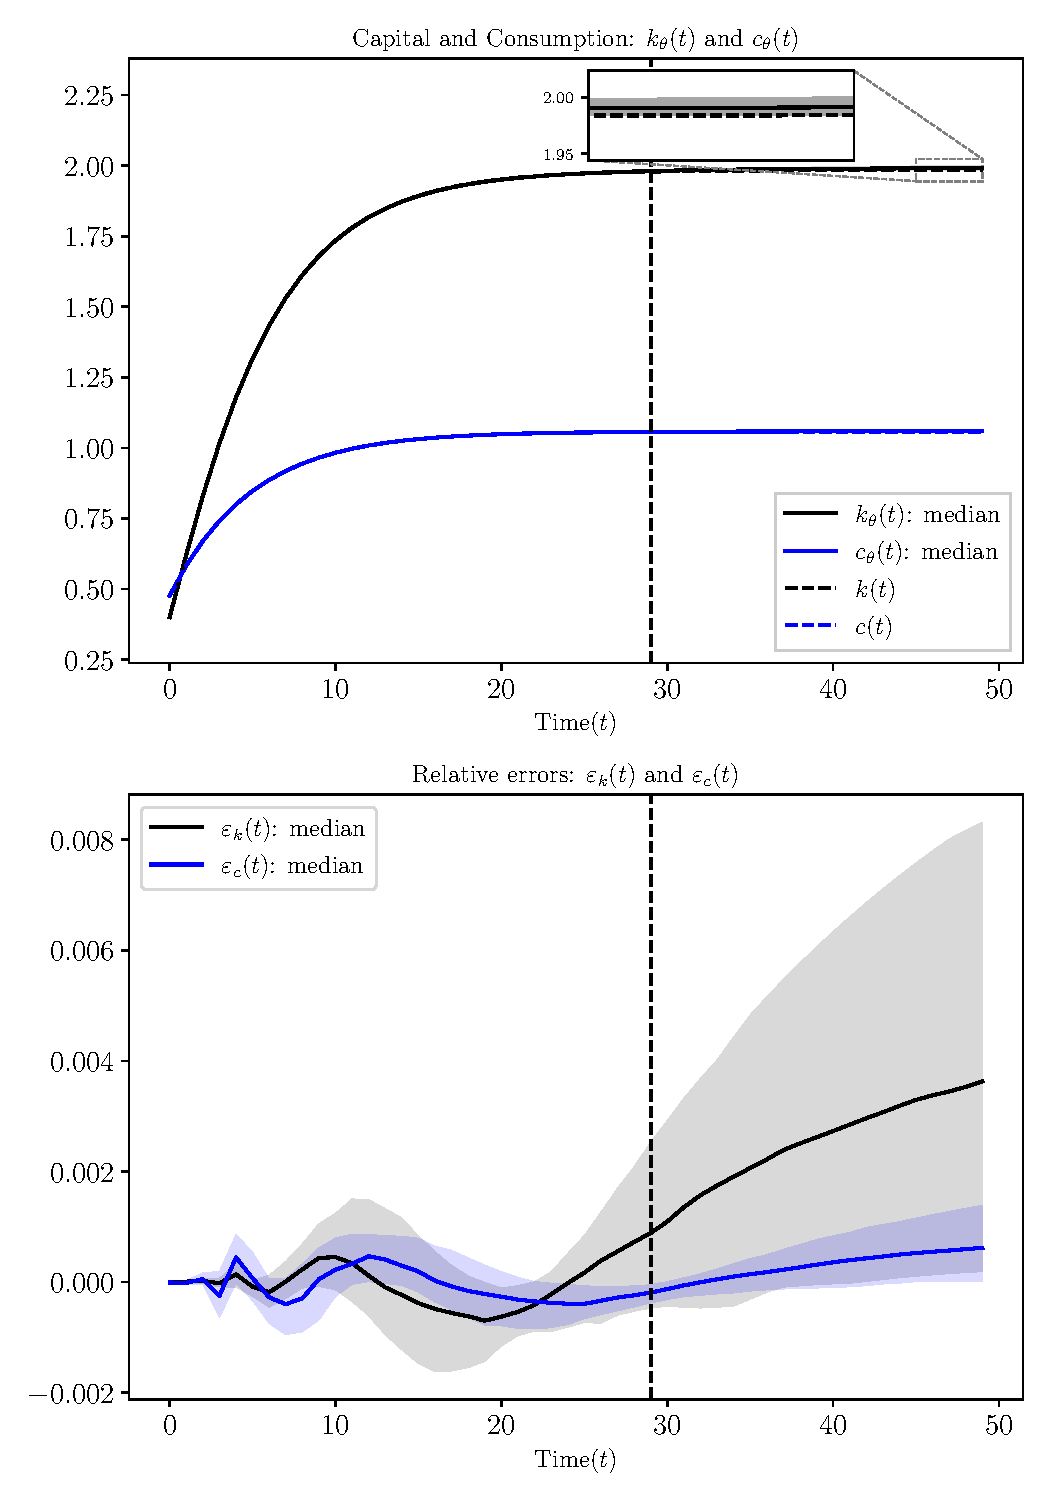
\includegraphics[width=0.6\textwidth]{figs/growth_sequential_g0.pdf}
				\hspace{25mm}
			\end{figure}
		\end{column}
	\end{columns}
\end{frame}

\begin{frame}{Neoclassical growth model with TFP growth: results}
	\begin{columns}
		\begin{column}{0.5\textwidth}
			% Content for the left column
			\begin{itemize}
				\item $g>0$ and $z(0) = 1$.
				\vspace{0.05in}
				\item $k_\theta(t) = e^{\phi t}
				NN_\theta(t)$, $\phi$ is "learnable".
				\vspace{0.05in}
				\item Results for $100$ different seeds (initialization of the parameters).
				\vspace{0.05in}
				\item Very accurate short- and medium-run approximation.
			\end{itemize}
		\end{column}
		\begin{column}{0.5\textwidth}
			\begin{figure}[t!]
				\centering
				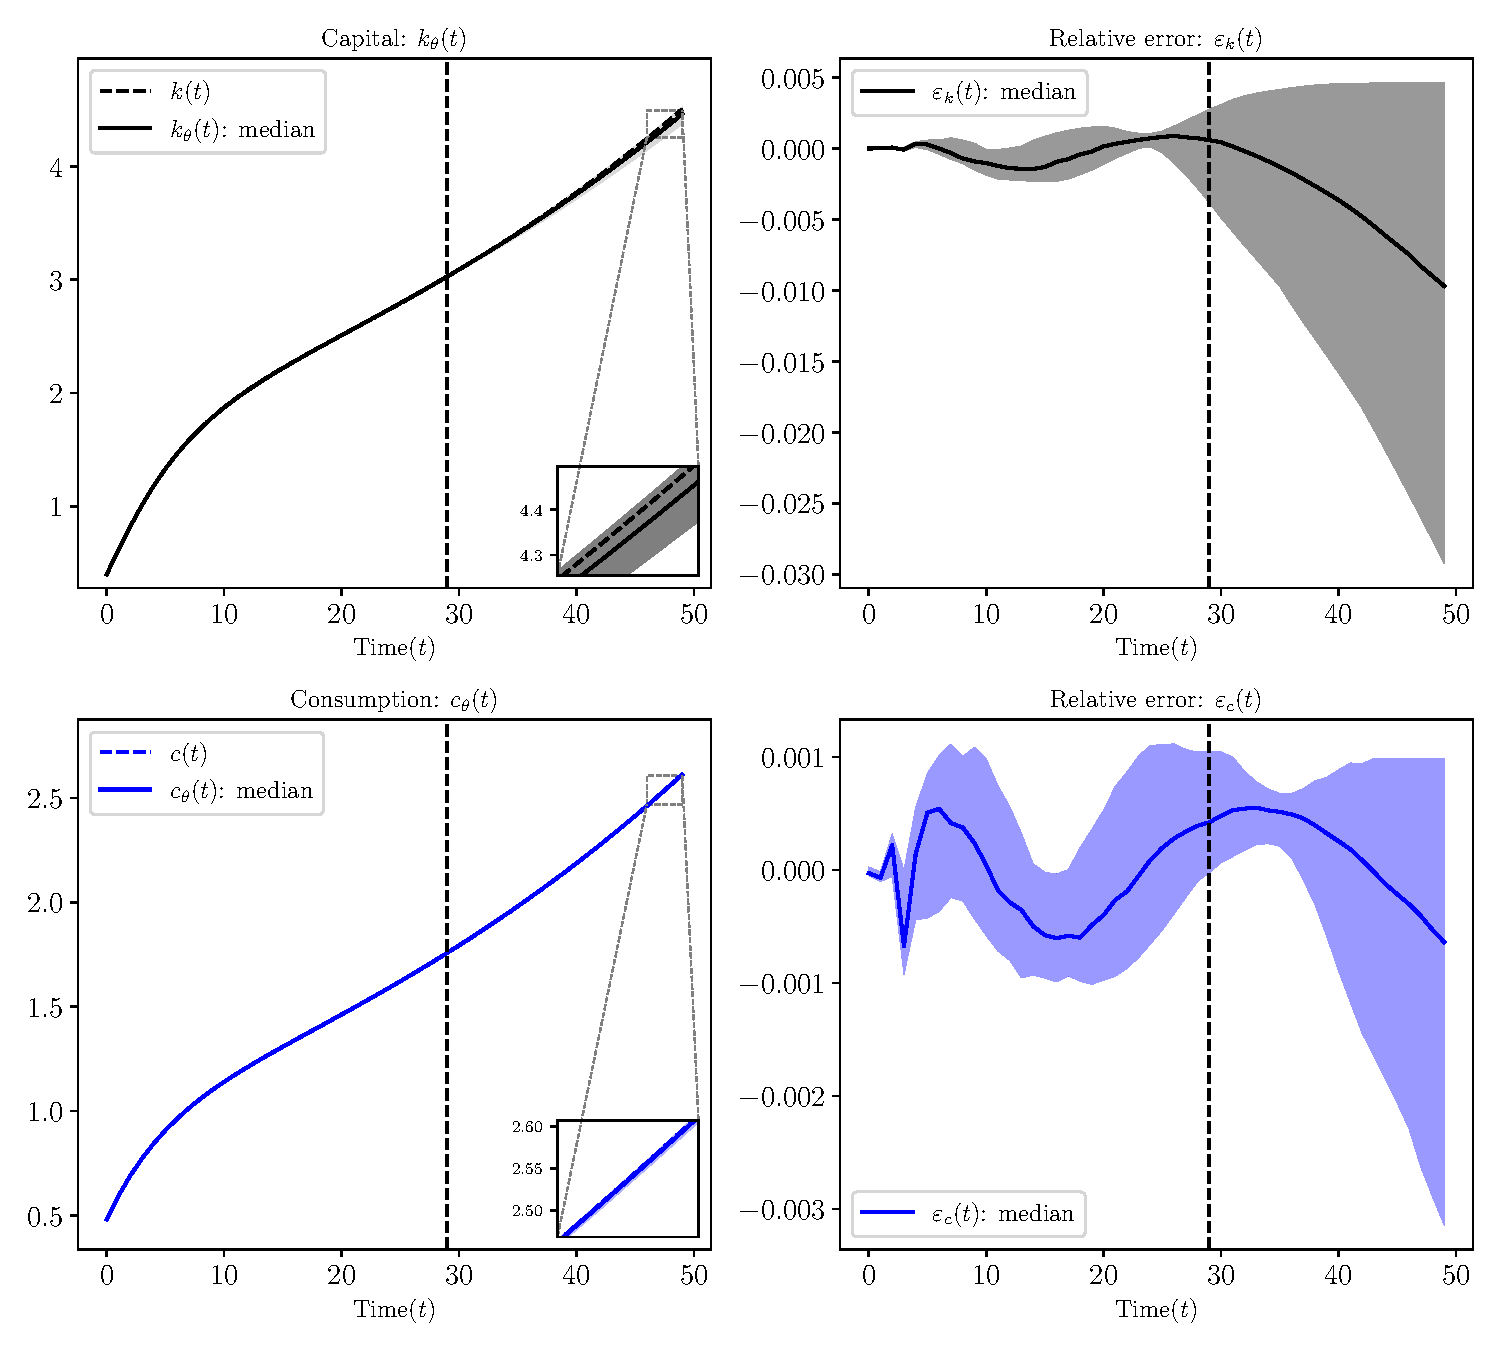
\includegraphics[width=\textwidth]{figs/growth_sequential_g_positive_ensemble.pdf}
				\vspace{-7mm}
			\end{figure}
		\end{column}
	\end{columns}
\end{frame}

\begin{frame}{But, ``in the long run, we are all dead"}

	\begin{columns}
	\begin{column}{0.5\textwidth}
		% Content for the left column
		\begin{itemize}
			\item So far, we have used long time-horizon $\mathcal{D} = \{0,1,\cdots,29\}$.
			\vspace{0.05in}
			\item In other methods, choosing the time-horizon $T$ is a challenge:
			\begin{itemize}
					\item Too large $\rightarrow$ accumulation of errors, and numerical instability. We don't have that problem.
				\item Too small $\rightarrow$ convergence to the steady state too quickly.
			\end{itemize}
			 \vspace{0.05in}
			\item An accurate short-run solution, even for a medium-sized $T$.
		\end{itemize}
	\end{column}
	\begin{column}{0.5\textwidth}
		\begin{figure}[t!]
			\centering
			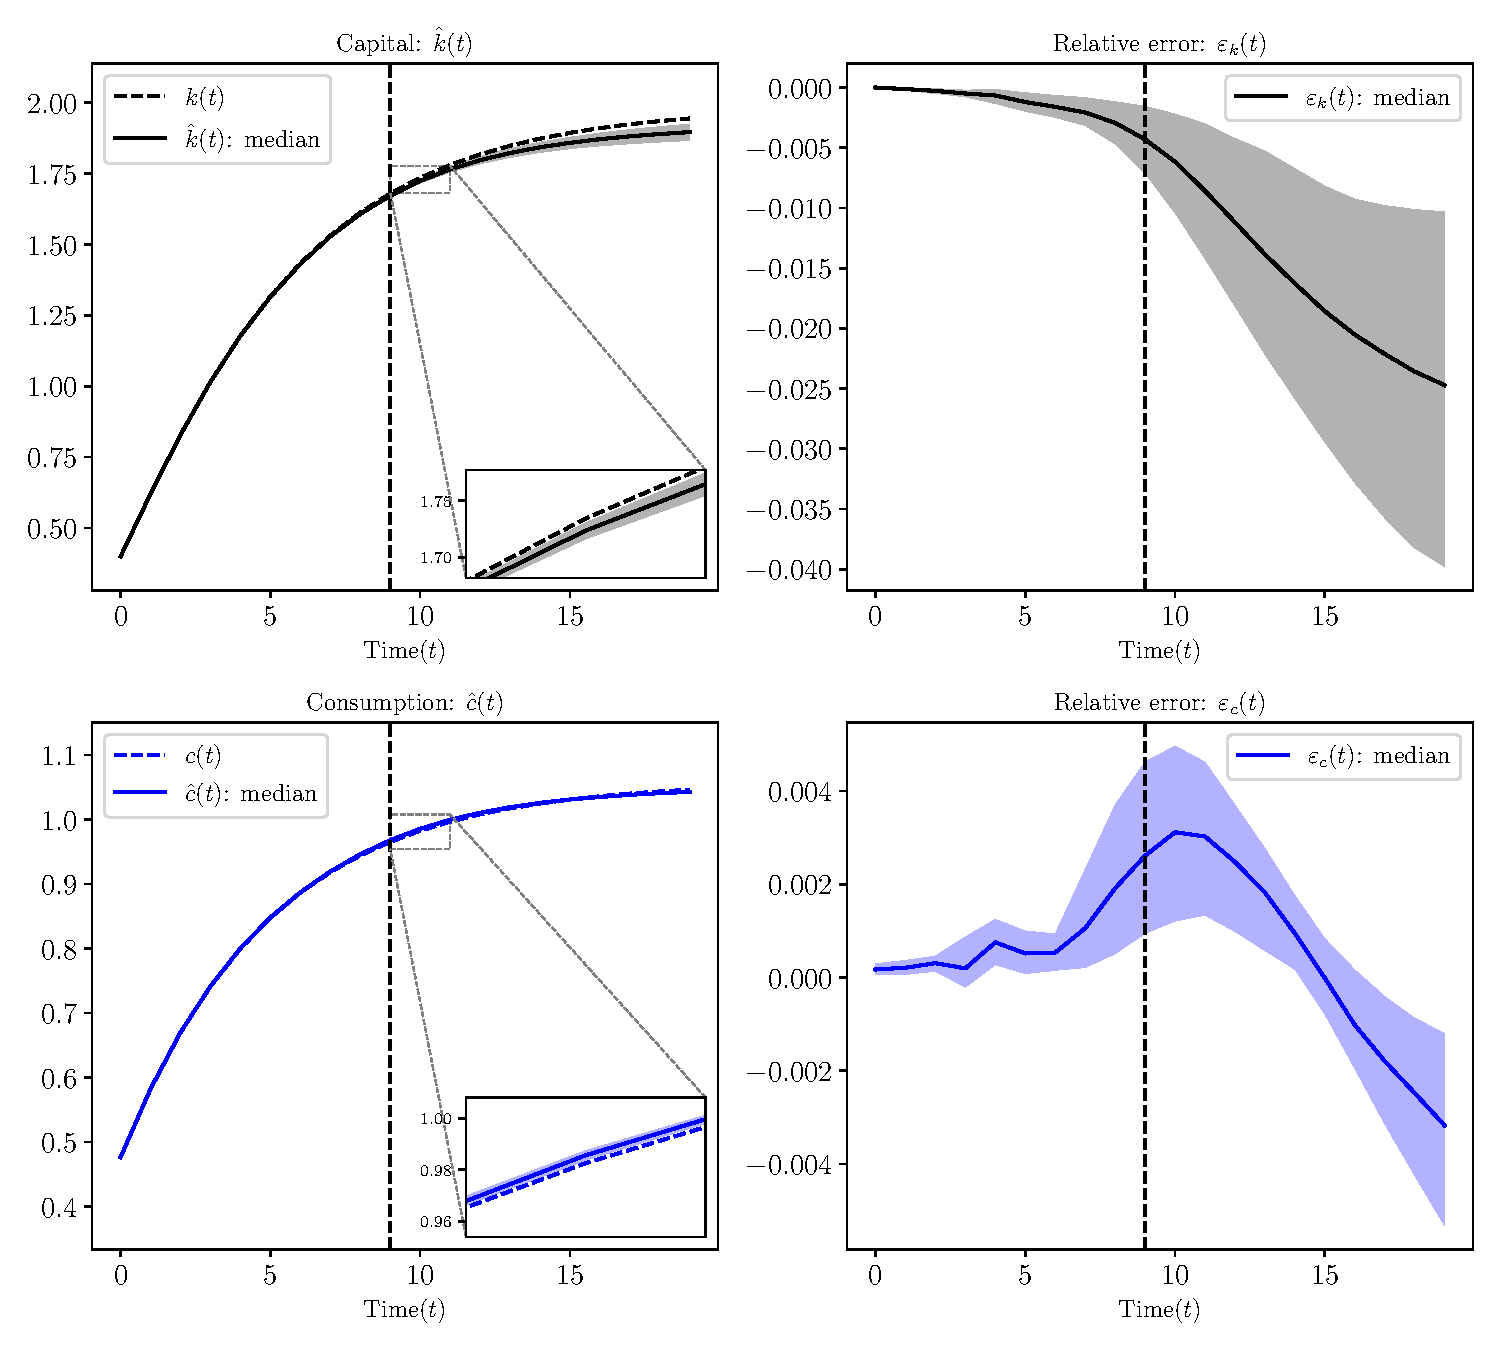
\includegraphics[width=\textwidth]{figs/growth_sequential_g0_t_max_9_ensemble.pdf}
			\vspace{-7mm}
		\end{figure}
	\end{column}
\end{columns}
\end{frame}


\begin{frame}{Neoclassical growth model: multiple steady-states and hysteresis}
	\begin{itemize}
	\item When there are multiple (saddle-path) steady states, each with its domain of attraction:
	\vspace{0.05in}
		\begin{itemize}
			\item Can the inductive bias detect there are multiple basins of attraction?
			\item How does the inductive
		bias move us toward the correct steady state for a given initial condition?
		\end{itemize}
	\vspace{0.05in}
	\item Consider a non-concave production function:
	\begin{align*}
		f(k) \equiv a \max\{k^\alpha, b_1k^\alpha-b_2\}
	\end{align*}
	\item Two steady-states $k_1^*$ and $k_2^*$.
	\vspace{0.05in}
	\item The same numerical procedure, different production function.
		\end{itemize}
\end{frame}

\begin{frame}{Neoclassical growth model with non-concave production function: results}
	\begin{figure}[t!]
		\centering
		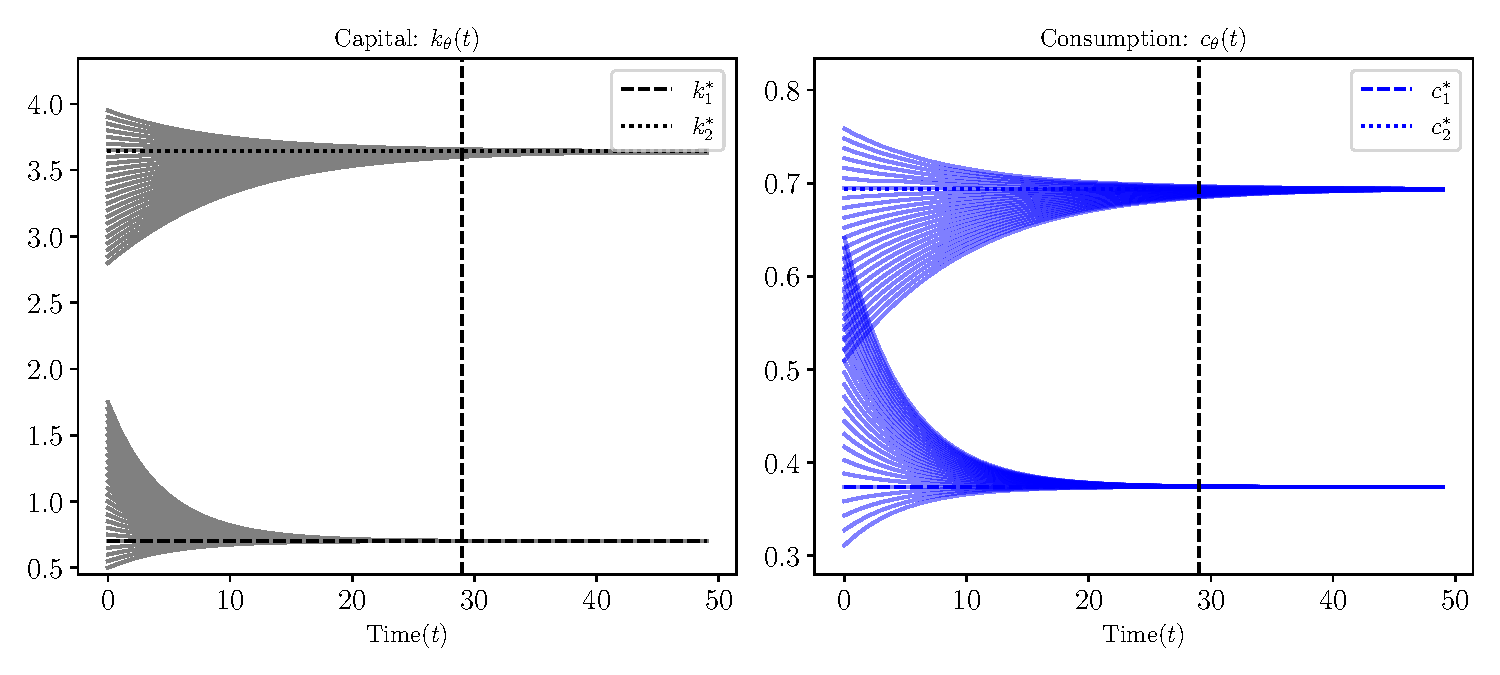
\includegraphics[width=0.75\textwidth]{figs/growth_sequential_multiple_steady_states_var_initial_k_0.pdf}
	\end{figure}
	\begin{itemize}
		\item Different initial conditions in $k_0 \in [0.5,1.75]\cup[2.75,4]$.
		\smallskip
		\item In the vicinity of $k_1^*$ and $k_2^*$ the paths converge to the right steady-states.
	\end{itemize}
\end{frame}


\begin{frame}{Deep learning is not the only option: kernels}
\begin{columns}
	\begin{column}{0.5\textwidth}
		% Content for the left column
			\begin{itemize}
			\item Deep learning might be too ``spooky".
			\smallskip
			\item We can use kernels, $K(\cdot,\cdot)$, instead of neural networks and control the RKHS norms. For instance:
			\begin{align*}
				\frac{dk}{dt} = \sum_{i=1}^N \alpha^k_i K(t,t_i), \quad \frac{dc}{dt} = \sum_{i=1}^N \alpha^c_i K(t,t_i)
			\end{align*}
			\item The same results, theoretical guarantees, very fast and robust.
		\end{itemize}
	\end{column}
	\begin{column}{0.5\textwidth}
		\begin{figure}[t!]
			\centering
			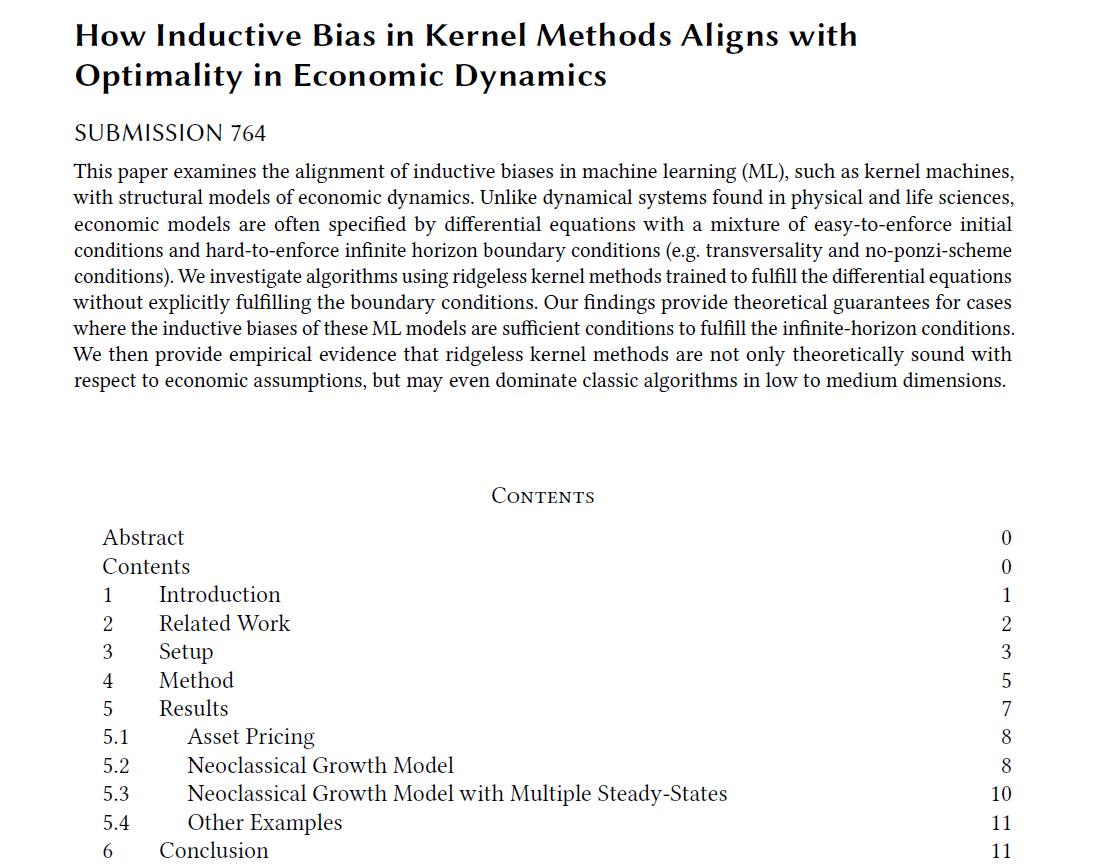
\includegraphics[width=0.9\textwidth]{figs/Kernel}
			\vspace{-7mm}
		\end{figure}
	\end{column}
\end{columns}

\end{frame}


\begin{frame}{Extensions in the paper}
	\begin{itemize}
		\item Sequential models:
		\begin{itemize}
			\item Shorter time-horizons.
			\smallskip
			\item Misspecification of growth.\\
			\smallskip
		\end{itemize}
		\smallskip
		\item Recursive neoclassical growth model
		\begin{itemize}
			\item Accurate short- and medium-run dynamics.
			\smallskip
			\item Accurate solutions even with TFP growth.
			\smallskip
			\item Deep learning solutions can go very wrong
			\begin{itemize}
				\smallskip
				\item We should use the information in the transversality condition to know what to approximate.
			\end{itemize} 
		\end{itemize}
	\end{itemize}
\end{frame}

\begin{frame}{Deep learning solutions can be misleading: approximating capital vs. consumption}
	\begin{columns}
		\begin{column}{0.5\textwidth}
			% Content for the left column
			\begin{itemize}
			\item Capital $k$ is the state variable.
			\smallskip
			\item Two options: approximating capital policy $k'_\theta(k)$ or $c_\theta(k)$
			\item left panels: results for $k'_\theta(k)$ approximation.
			\smallskip
			\item Right panels: results for $c_\theta(k)$ approximation.
			\smallskip
			\item Only the left panel results are correct. 
			$k'_\theta(k)$ has a fixed point at the right steady state.
			\smallskip
			\item However, the wrong solution leads to lower Euler residuals.
			\end{itemize}
		\end{column}
		\begin{column}{0.75\textwidth}
			\begin{figure}[t!]
				\centering
				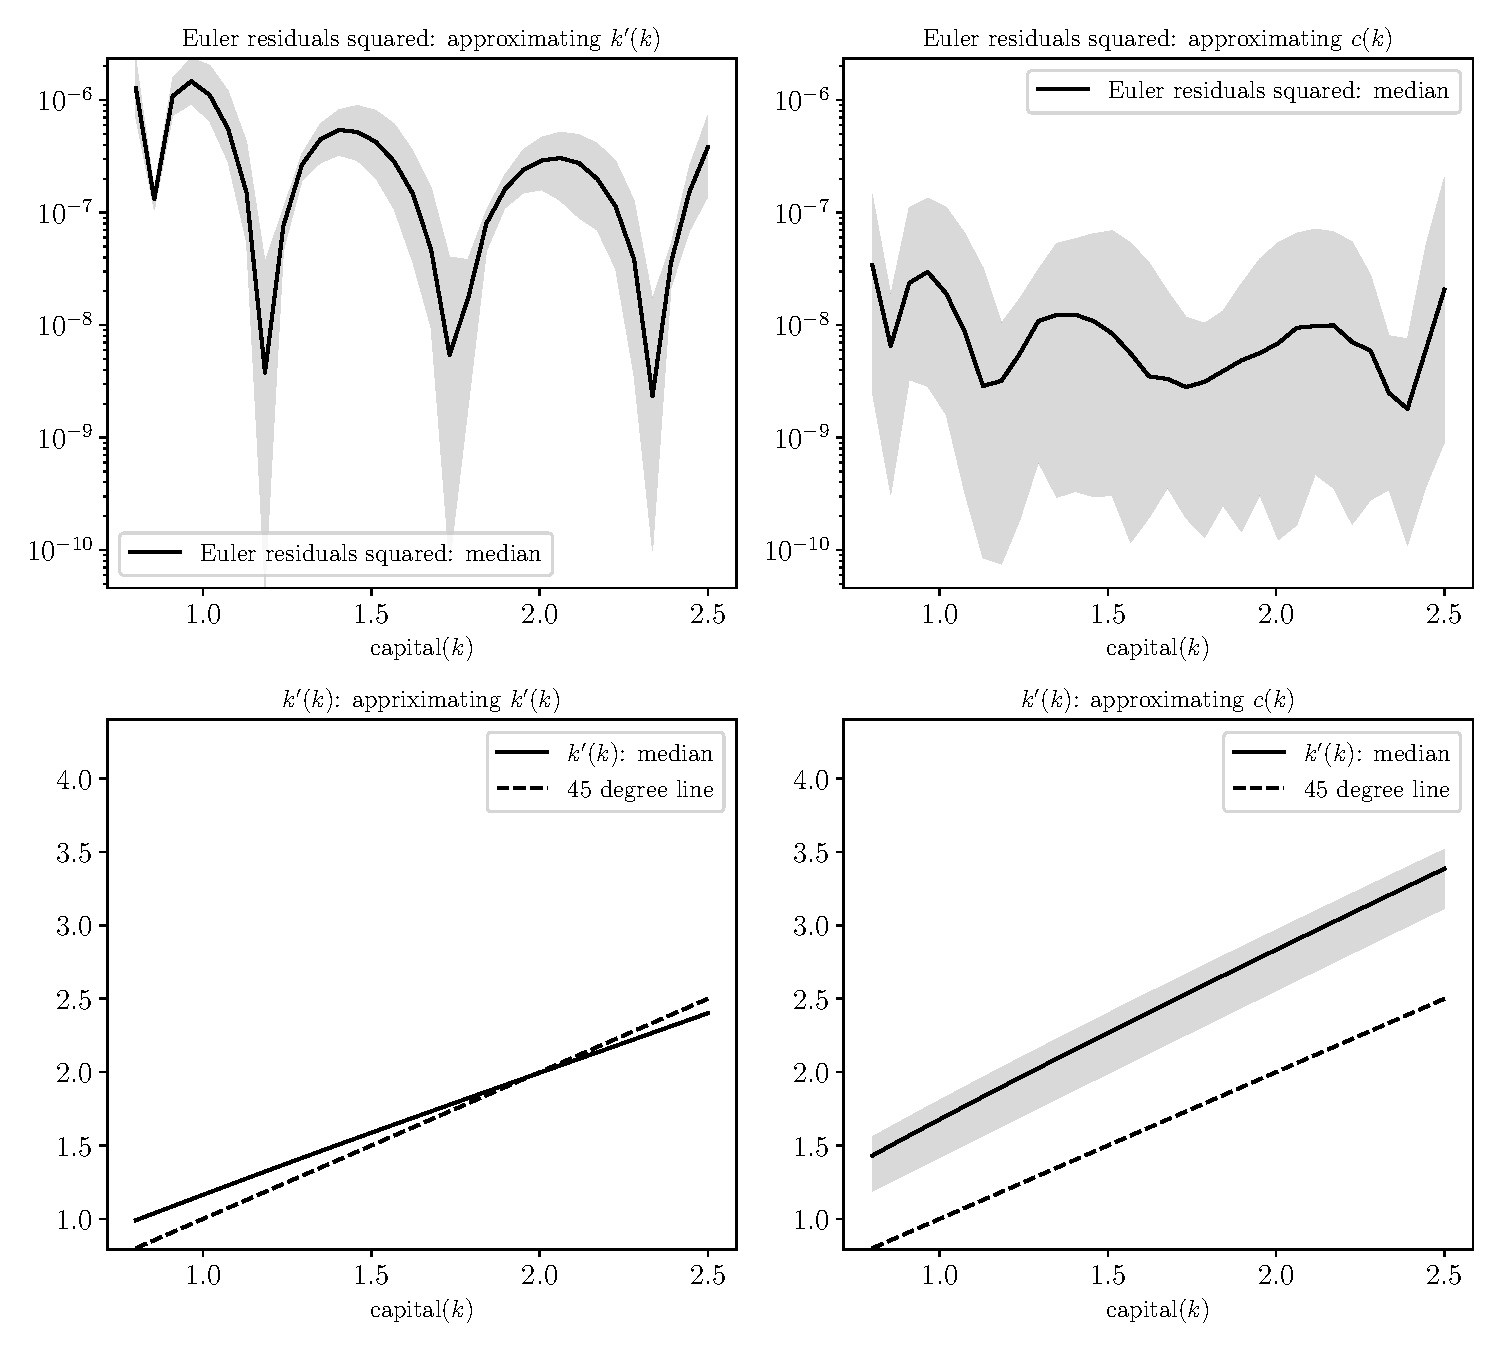
\includegraphics[width=0.7\textwidth]{figs/growth_recursive_g0_euler_residuals_grid.pdf}
				\hspace{32mm}
			\end{figure}
		\end{column}
	\end{columns}
	\end{frame}
	


\begin{frame}{Conclusion}
	\begin{itemize}
		\item Long-run (\emphcolor{global}) conditions can be replaced with appropriate regularization (\emphcolor{local}) to achieve optimal solutions, hence the title of the paper.
		\vspace{0.1in}
		\item Inductive bias provides a foundation for modeling forward-looking behavioral agents with self-consistent expectations.
	\end{itemize}
\end{frame}

\begin{frame}{Discussion: where to go from here?}
	\begin{itemize}
		\item Can inductive bias/regularization be thought of as an equilibrium selection device?
		\begin{itemize}
			\item In this paper it is used to select solutions.
		\end{itemize}
		\smallskip
		\item This method (mostly the kernel method) can be used for sampling high-dimensional state spaces when there is stochasticity. 
		\begin{itemize}
		\item Solve the deterministic in short-run and use the points as sample of the state-space.
		\smallskip
		\item Then solve the stochastic problem.
		\end{itemize}
		%if we are about to translate economic dynamic models into an ERM, can regularization act as an equilibrium device? Think about it, ERM in statistical learning or machine learning is about two things: uniform of law of large numbers and capacity control (so what are going to do about this capacity control regularization)
	\end{itemize}
\end{frame}
\section{Appendix}


\end{document}
